\documentclass{article}
\usepackage{
	amsmath,			% Math Environments
	amssymb,			% Extended Symbols
	enumerate,		    % Enumerate Environments
	graphicx,			% Include Images
        minted,
        caption,
        subcaption,
        booktabs
}
\usepackage[norsk]{babel}
\usepackage[T1]{fontenc}
\usepackage{hyperref}
\hypersetup{breaklinks=true,colorlinks=true,linkcolor=blue,citecolor=blue,filecolor=magenta,urlcolor=blue}
\bibliographystyle{apalike}

\title{MAT3100 - Oblig 1}
\author{August Femtehjell}
\date{February 2024}

\renewcommand{\thesection}{Oppgave \arabic{section}}
\renewcommand{\thesubsection}{\arabic{section}\alph{subsection})}
\renewcommand{\thesubsubsection}{Besvarelse}

\title{MAT1020 - Oblig 1\\Matematikk og bærekraftig forvaltning}
\author{August Femtehjell}
\date{March 2024}

\begin{document}

\maketitle

\noindent
All koden for denne obligen er tilgjengelig på \url{https://github.com/augustfe/MAT1020}, skrevet i \verb|Python|.

\section{}
I denne oppgaven skal du gjøre en statistisk analyse av kapasitetsfaktordataene.

\subsection{}
Plot alle dataseriene (gjerne som illustrative utsnitt av tidsseriene), og se om det er forskjeller mellom årstidene. Hva kan du si om solkraft nord og sør i Europa og vindkraft på de forskjellige stedene i Norge?

\subsubsection{}
Etter som solkapasitetene er gitt ved maskimalverdier klokken 12, er vi nødt til å gjøre justeringer for å få representative daglige verdier.
Hvis vi antar at gjennomsnitts solkapasiteten er gitt ved halvparten av maks, og at det er 12 timer med sol hver dag, ganger vi de gitte solkapasitetene med $\frac{1}{4}$ for å justere.
Det kan diskuteres hvorvidt dette er en representativ måte å bearbeide dataen, spesielt med tanke på at antall soltimer i løpet av et døgn varierer med tiden av året, og lokasjon.
Oslo ligger for eksempel på rundt 1700 timer med sol hvert år, mens Athen ligger på omtrent 2800 \cite{soltimer}.

For å få et inntrykk av hva slags data vi jobber med, plotter jeg tidsseriene uten videre justeringer i \autoref{fig:rene_tidserier}, ved hjelp av \verb|Pandas| sitt \verb|DataFrame|.
Som en kan se, er dette ikke særlig illustrativt, på grunn av de store daglige svingningene, annet enn at solkapasitet angivelig varierer med årstid.

\begin{figure}[ht]
\centering
\begin{subfigure}{.5\textwidth}
    \centering
    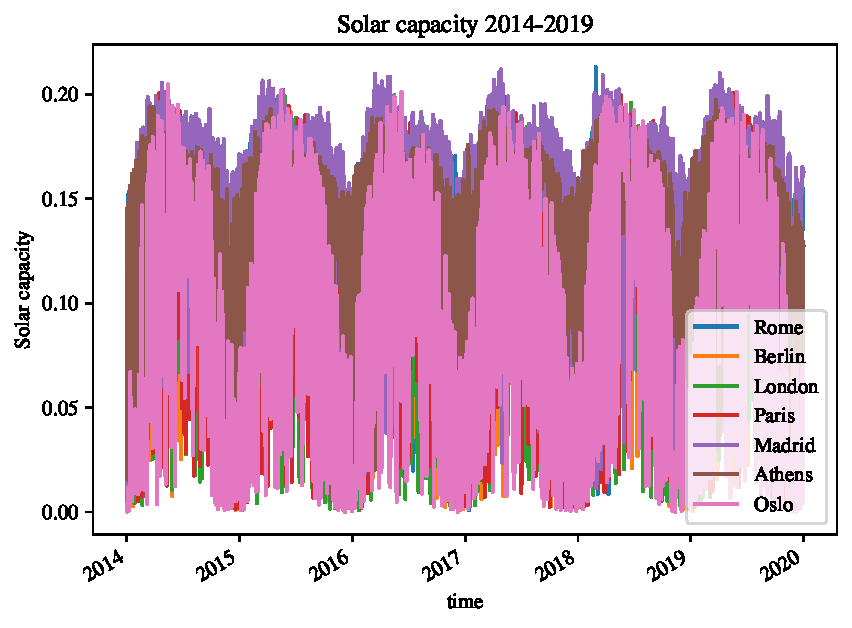
\includegraphics[width=\linewidth]{oblig/figures/Solar/Solar capacity 2014-2019.pdf}
    \caption{Solkapasitet}
    \label{fig:ren_sol}
\end{subfigure}%
\begin{subfigure}{.5\textwidth}
    \centering
    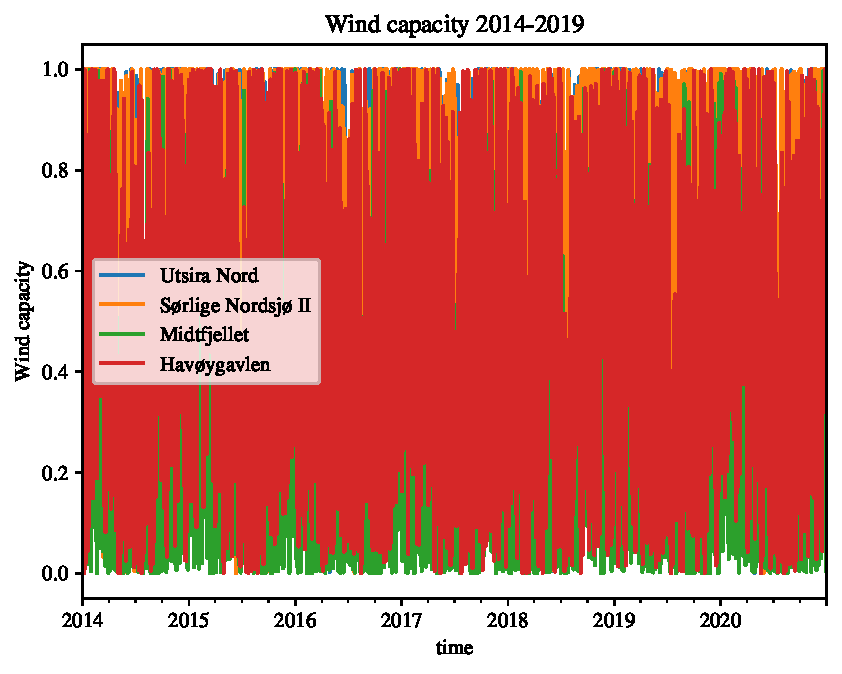
\includegraphics[width=\linewidth]{oblig/figures/Wind/Wind capacity 2014-2019.pdf}
    \caption{Vindkapasitet}
    \label{fig:ren_vind}
\end{subfigure}
\caption{Tidsserier for sol- og vindkapasitet.}
\label{fig:rene_tidserier}
\end{figure}

For å få et bedre bilde, velger jeg derfor å benytte meg av et løpende gjennomsnitt på 30 dager, ved \verb|DataFrame.rolling(30).mean|, for å luke ut de mindre daglige svingingene.
I tillegg, så velger jeg å fokusere på et enkelt år, hvor 2017 er valgt arbitrært.
I \autoref{fig:rolling_2017_sol} kan vi nå tydeligere se at solkapasitetene varierer sterkt fra by til by, med høyere kapasitet i sør og lavere i nord.
Med vindkapasitetene i \autoref{fig:rolling_2017_vind}, skiller Midtfjellet seg sterkt ut fra de andre lokasjonene.

\begin{figure}[ht]
\centering
\begin{subfigure}{.5\textwidth}
    \centering
    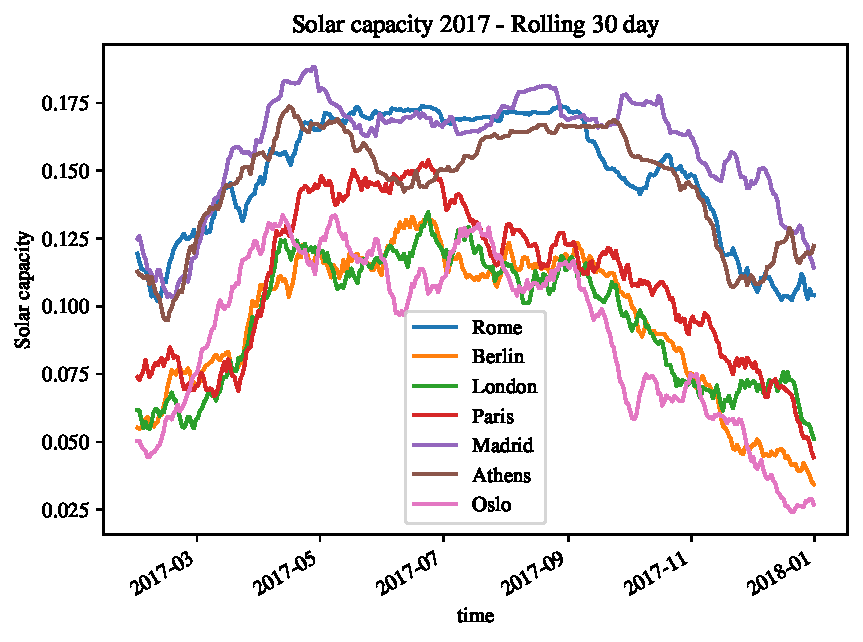
\includegraphics[width=\linewidth]{oblig/figures/Solar/Solar capacity 2017 - Rolling 30 day.pdf}
    \caption{Solkapasitet}
    \label{fig:rolling_2017_sol}
\end{subfigure}%
\begin{subfigure}{.5\textwidth}
    \centering
    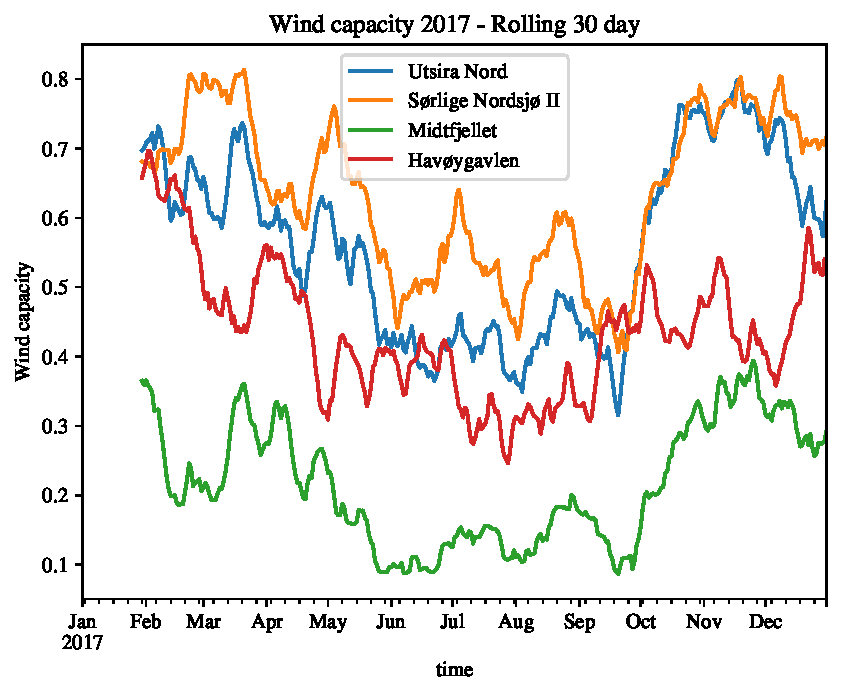
\includegraphics[width=\linewidth]{oblig/figures/Wind/Wind capacity 2017 - Rolling 30 day.pdf}
    \caption{Vindkapasitet}
    \label{fig:rolling_2017_vind}
\end{subfigure}
\caption{Løpende gjennomsnitt over 30 dager, for sol- og vindkapasitet i 2017.}
\label{fig:rolling_2017}
\end{figure}

\newpage
\subsection{}
Finn gjennomsnittlig kapasitetsfaktor for hver sol- og vind-dataserie. Husk å omforme sol-dataene til representative daglige verdier.

\subsubsection{}
De gjennomsnittlige kapasitetsfaktorene er oppgitt i \autoref{tab:gjennomsnitt_tabell}, merk at soldataen allerede er justert til mer representative daglige verdier.
Verdiene er utregnet ved \verb|DataFrame.mean|.

\begin{table}[h]
\centering
\subfloat[Solkraft]{
    \begin{tabular}{|l|r|}
    \hline
    Roma     & 0.138063 \\
    \hline
    Berlin   & 0.098143 \\
    \hline
    London   & 0.096166 \\
    \hline
    Paris    & 0.107171 \\
    \hline
    Madrid   & 0.149532 \\
    \hline
    Athen   & 0.139312 \\
    \hline
    Oslo     & 0.087412 \\
    \hline
    \end{tabular}
}
\qquad
\subfloat[Vindkraft]{
    \begin{tabular}{|l|r|}
    \hline
    Utsira Nord          & 0.571073 \\
    \hline
    Sørlige Nordsjø II   & 0.640919 \\
    \hline
    Midtfjellet          & 0.243222 \\
    \hline
    Havøygavlen          & 0.469817 \\
    \hline
    \end{tabular}
    }
\caption{Gjennomsnittlige kapasitetsfaktorer per lokasjon og teknologi.}
\label{tab:gjennomsnitt_tabell}
\end{table}

Her blir forskjellene mellom regionene mer markante, blant annet ved at madrid i sør har en $1.71$ ganger høyere gjennomsnittlig kapasitetsfaktor enn Oslo i Nord, og at off-shore installasjonen Sørlige Nordsjø II har en $2.64$ ganger høyere kapasitetsfaktor enn Midtfjellet.

\newpage
\subsection{}
Finn varians og standardavvik for kapasitetsfaktorene i hver lokasjon og hver teknologi (det vil si, sol og vind)

\subsubsection{}
Standardavvikene er oppgitt i \autoref{tab:std_tabell}.
Standardavviket i Oslo er betydelig høyere enn for eksempel Athen, som gir mening ettersom det er betydelig mindre sol i Oslo om vinteren enn det er i Athen.
Solkraft har dog betydelig lavere standardavvik enn vindkraft. Verdiene er utregnet ved \verb|DataFrame.std|.

\begin{table}[h]
\centering
\subfloat[Solkraft]{
\begin{tabular}{|l|r|}
    \hline
    Roma & 0.043663 \\
    \hline
    Berlin & 0.054475 \\
    \hline
    London & 0.053795 \\
    \hline
    Paris & 0.057088 \\
    \hline
    Madrid & 0.046485 \\
    \hline
    Athen & 0.039253 \\
    \hline
    Oslo & 0.061271 \\
    \hline
\end{tabular}
}
\qquad
\subfloat[Vindkraft]{
\begin{tabular}{|l|r|}
    \hline
    Utsira Nord & 0.330635 \\
    \hline
    Sørlige Nordsjø II & 0.315474 \\
    \hline
    Midtfjellet & 0.266767 \\
    \hline
    Havøygavlen & 0.315342 \\
    \hline
\end{tabular}
}
\caption{Standardavvik for kapasitetsfaktorer per lokasjon og teknologi.}
\label{tab:std_tabell}
\end{table}

Variansene er oppgitt langs diagonalene av \autoref{fig:correlation}, generert ved \verb|DataFrame.cov|.

\begin{figure}[h]
\centering
\begin{subfigure}{.5\textwidth}
    \centering
    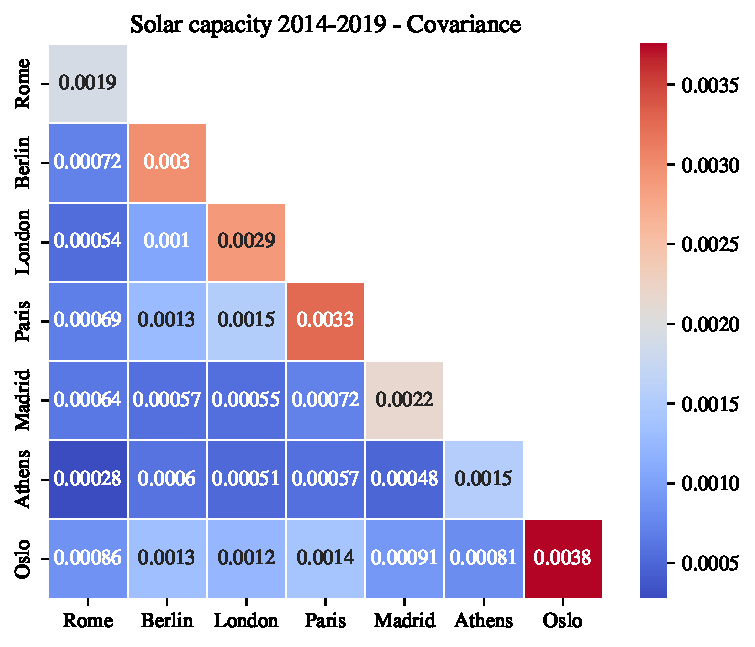
\includegraphics[width=\linewidth]{oblig/figures/Solar/Solar capacity 2014-2019 - Covariance.pdf}
    \caption{Solkapasitet}
    \label{fig:cov_sol}
\end{subfigure}%
\begin{subfigure}{.5\textwidth}
    \centering
    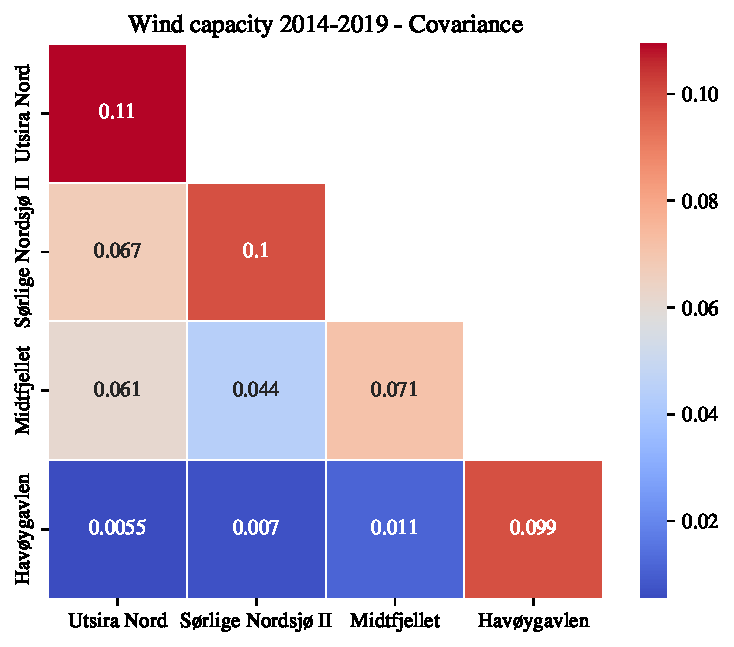
\includegraphics[width=\linewidth]{oblig/figures/Wind/Wind capacity 2014-2019 - Covariance.pdf}
    \caption{Vindkapasitet}
    \label{fig:cov_vind}
\end{subfigure}
\caption{Kovarians mellom lokasjoner, for hver teknologi.}
\label{fig:covariance}
\end{figure}



\subsection{}
Finn kovariansen til kapasitetsfaktorene mellom lokasjoner for vind. Hva blir korrelasjonene?

\subsubsection{}
I \autoref{fig:cov_vind} kan vi lese at det er absolutt minst korrelasjon mellom Havøygavlen og de andre.
Dette gir mening, ettersom Havøygavlen ligger i Finnmark, mens eksempelvis Midtfjellet ligger på vestlandet.
Korrelasjonene er oppgitt i \autoref{fig:corr_vind}.

\begin{figure}[h]
\centering
\begin{subfigure}{.5\textwidth}
    \centering
    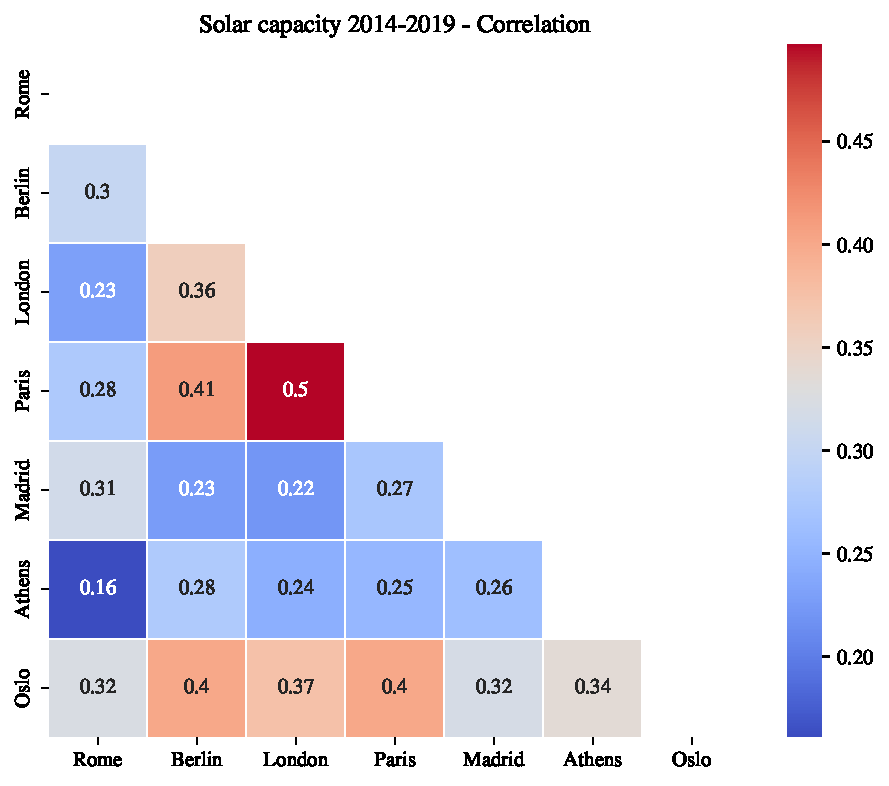
\includegraphics[width=\linewidth]{oblig/figures/Solar/Solar capacity 2014-2019 - Correlation.pdf}
    \caption{Solkapasitet}
    \label{fig:corr_sol}
\end{subfigure}%
\begin{subfigure}{.5\textwidth}
    \centering
    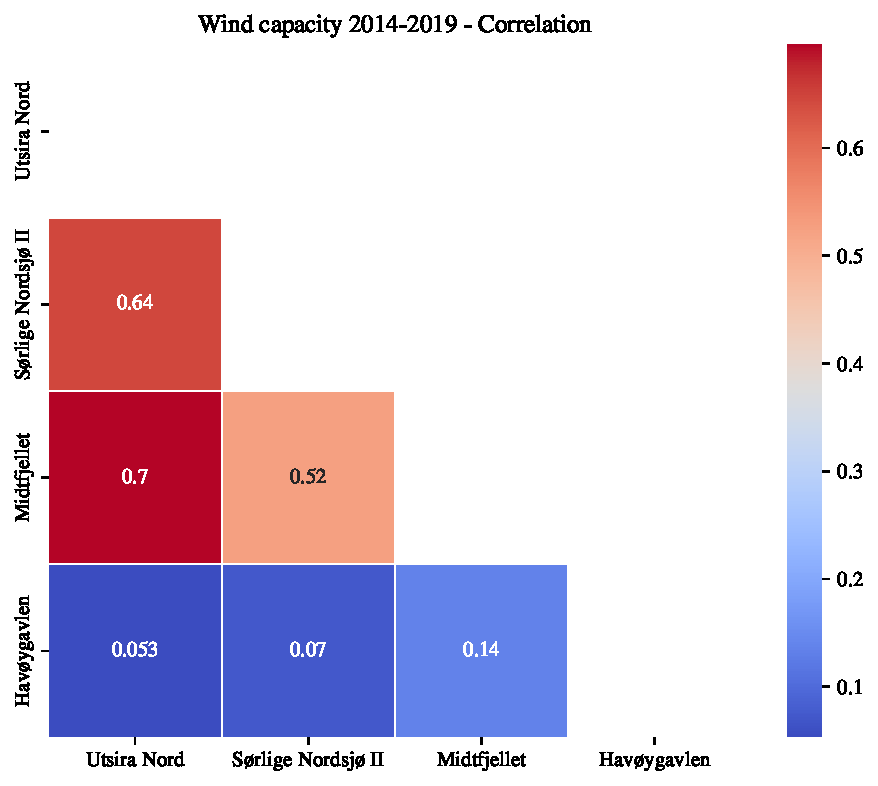
\includegraphics[width=\linewidth]{oblig/figures/Wind/Wind capacity 2014-2019 - Correlation.pdf}
    \caption{Vindkapasitet}
    \label{fig:corr_vind}
\end{subfigure}
\caption{Korrelasjoner mellom lokasjoner, for hver teknologi.}
\label{fig:correlation}
\end{figure}

\subsection{}
Finn kovariansen til kapasitetsfaktorene mellom lokasjoner for sol. Hva blir korrelasjonene?

\subsubsection{}
I \autoref{fig:cov_sol} kan vi lese av kovariansen til solkapasitetene mellom byene i Europa.
Det er betraktelig lavere kovarians i denne settingen, dog høyere mellom byer som Paris og London.
Dette gir mening ettersom det er omtrentlige 344km mellom de, mot 2600km mellom Oslo og Athen.
Korrelasjonene er oppgitt i \autoref{fig:corr_sol}.

\subsection{}
Finn varians-kovariansmatrisen for kapasitetsfaktorene til sol og for kapasitetsfaktorene til vind.

\subsubsection{}
For ordens skyld er varians-kovariansmatrisen for sol oppgitt i \autoref{tab:var_cov_sol} og vind i \autoref{tab:var_cov_vind}. Merk at dette ble svært lite lesbart, og inneholder den samme informasjonen som \autoref{fig:covariance}. Verdiene er fremdeles generert ved \verb|DataFrame.cov|.

\begin{table}[h]
\centering
$$
\begin{bmatrix}
0.001906 & 0.000715 & 0.000539 & 0.000689 & 0.000637 & 0.000276 & 0.000863 \\
0.000715 & 0.002968 & 0.001045 & 0.001277 & 0.000571 & 0.000595 & 0.001335 \\
0.000539 & 0.001045 & 0.002894 & 0.001526 & 0.000551 & 0.000515 & 0.001232 \\
0.000689 & 0.001277 & 0.001526 & 0.003259 & 0.000720 & 0.000568 & 0.001400 \\
0.000637 & 0.000571 & 0.000551 & 0.000720 & 0.002161 & 0.000479 & 0.000908 \\
0.000276 & 0.000595 & 0.000515 & 0.000568 & 0.000479 & 0.001541 & 0.000807 \\
0.000863 & 0.001335 & 0.001232 & 0.001400 & 0.000908 & 0.000807 & 0.003754 \\
\end{bmatrix}
$$
\caption{Varians-kovariansmatrisen for kapasitetsfaktorene til sol, i samme rekkefølge som \autoref{tab:gjennomsnitt_tabell}.}
\label{tab:var_cov_sol}
\end{table}

\begin{table}[h]
\centering
$$
\begin{bmatrix}
0.109319 & 0.067227 & 0.061392 & 0.005485 \\
0.067227 & 0.099524 & 0.044098 & 0.006990 \\
0.061392 & 0.044098 & 0.071165 & 0.011390 \\
0.005485 & 0.006990 & 0.011390 & 0.099441 \\
\end{bmatrix}
$$
\caption{Varians-kovariansmatrisen for kapasitetsfaktorene til vind, i samme rekkefølge som \autoref{tab:gjennomsnitt_tabell}.}
\label{tab:var_cov_vind}
\end{table}





\bibliography{references}
\end{document}
